\documentclass[tikz, border=10mm]{standalone}
\usetikzlibrary{calc}

\begin{document}
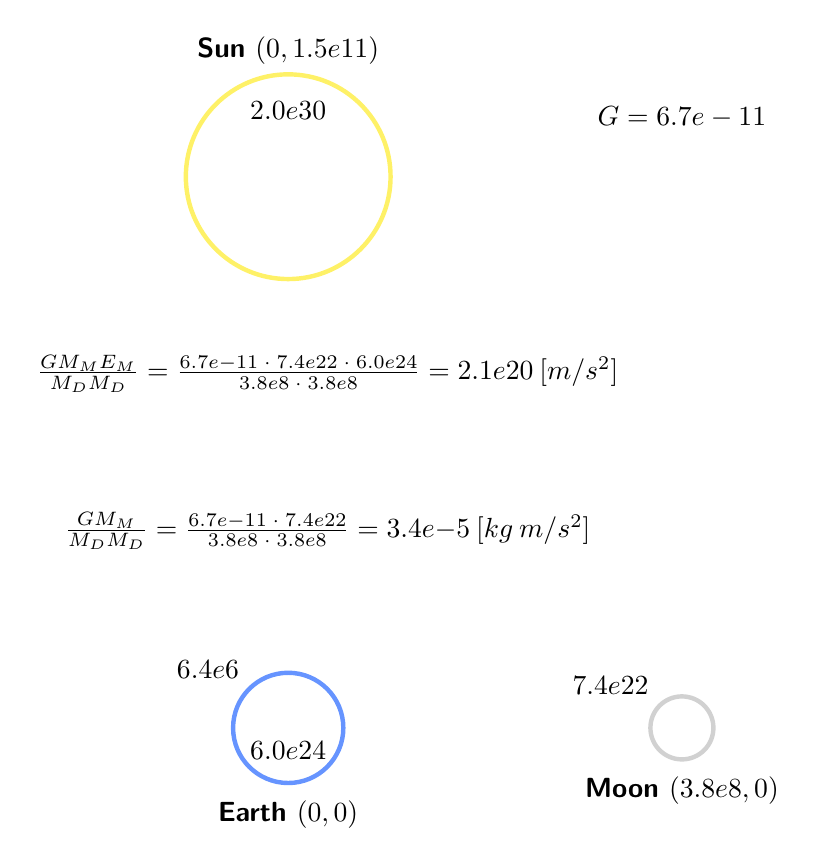
\begin{tikzpicture}

    % -------------------------------------------------------------
    % 1. DEFINE COORDINATES & SYSTEM VARIABLES
    % -------------------------------------------------------------
    % Adjust these values to scale the diagram as needed
    \def\dm{5.0}    % Earth distance from Moon along x-axis
    \def\de{4.0}    % Earth distance from Moon along x-axis
    \def\ds{0}   % Sun x-coordinate
    \def\dt{7.0}    % Sun y-coordinate

    % Define positions based on your vector layout
    \coordinate (Moon)  at (\dm,0);
    \coordinate (Earth) at (0, 0);
    \coordinate (Sun)   at (\ds, \dt);

    % Body sizes (radii)
    \def\rMoon{0.3}
    \def\rEarth{0.6}
    \def\rSun{1.2}

    % --- SUN ---
    % Shaded orange/yellow sphere
%   \shading[ball color=orange!80!yellow] (Sun) circle (\rSun);
    % Outer glow/rays effect
    \draw[yellow!90!orange, ultra thick, opacity=0.6] (Sun) circle (\rSun + 0.1);
    \node[above=1.3cm, font=\sffamily\bfseries] at (Sun) {Sun $(0, 1.5e11)$};
    \node[above=0.6cm, font=\sffamily\bfseries] at (Sun) {$2.0e30$};

    % --- EARTH ---
    % Shaded blue/cyan sphere
%   \shading[ball color=blue!70!cyan] (Earth) circle (\rEarth);
    \draw[blue!70!cyan, ultra thick, opacity=0.6] (Earth) circle (\rEarth + 0.1);
    \node[below=0.8cm, font=\sffamily\bfseries] at (Earth) {Earth $(0, 0)$};
    \node[above left=0.5cm, font=\sffamily\bfseries] at (Earth) {$6.4e6$};
    \node[below=0.05cm, font=\sffamily\bfseries] at (Earth) {$6.0e24$};

    % --- MOON ---
    % Shaded gray sphere at the origin
%   \shading[ball color=black!30!white] (Moon) circle (\rMoon);
    \draw[black!30!white, ultra thick, opacity=0.6] (Moon) circle (\rMoon + 0.1);
    \node[below=0.5cm, font=\sffamily\bfseries] at (Moon) {Moon $(3.8e8,0)$};
    \node[above=7.5cm, font=\sffamily\bfseries] at (Moon) {$G=6.7e-11$};
    \node[above left=0.3cm, font=\sffamily\bfseries] at (Moon) {$7.4e22$};

    \node[font=\sffamily\bfseries] at (0.5,2.5) {$\frac{G M_M}{M_D M_D}=\frac{6.7e-11\hspace{0.75mm}\cdot\hspace{0.75mm}7.4e22}{3.8e8\hspace{0.75mm}\cdot\hspace{0.75mm}3.8e8}=3.4e{-}5\hspace{0.75mm}[kg\hspace{0.75mm}m/s^2]$};

    \node[font=\sffamily\bfseries] at (0.5,4.5) {$\frac{G M_M E_M}{M_D M_D}=\frac{6.7e-11\hspace{0.75mm}\cdot\hspace{0.75mm}7.4e22\hspace{0.75mm}\cdot\hspace{0.75mm}6.0e24}{3.8e8\hspace{0.75mm}\cdot\hspace{0.75mm}3.8e8}=2.1e20\hspace{0.75mm}[m/s^2]$};
%   \node[font=\sffamily\bfseries] at (0.5,4.5) {$\frac{G M_M E_M}{M_D M_D}=\frac{6.7e-11\hspace{0.75mm}\cdot\hspace{0.75mm}7.4e22\hspace{0.75mm}\cdot\hspace{0.75mm}6.0e24}{3.8e8\hspace{0.75mm}\cdot\hspace{0.75mm}3.8e8}=3.4e{-}5\hspace{0.75mm}[m/s^2]$};

\end{tikzpicture}
\end{document}
